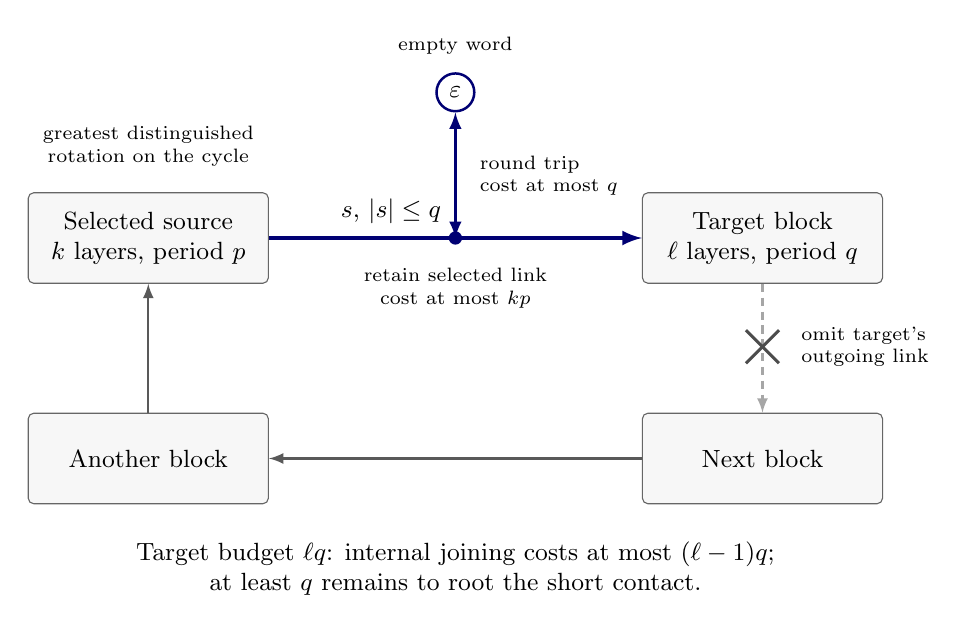
\begin{tikzpicture}[font=\small,>=latex,
  block/.style={draw=black!60,rounded corners=2pt,fill=black!3,
    minimum width=3.05cm,minimum height=1.15cm,align=center,inner sep=5pt},
  link/.style={->,draw=black!65,line width=.8pt},
  selected/.style={->,draw=blue!45!black,line width=1.4pt}]
  \node[block] (source) at (0,2.8)
    {Selected source\\$k$ layers, period $p$};
  \node[block] (target) at (7.8,2.8)
    {Target block\\$\ell$ layers, period $q$};
  \node[block] (next) at (7.8,0)
    {Next block};
  \node[block] (last) at (0,0)
    {Another block};

  \draw[selected] (source.east) -- (target.west)
    node[midway,below=7pt,align=center,font=\scriptsize]
      {retain selected link\\cost at most $kp$};
  \draw[link] (next.west) -- (last.east);
  \draw[link] (last.north) -- (source.south);

  \draw[->,draw=black!35,densely dashed,line width=.8pt]
    (target.south) -- (next.north);
  \draw[black!70,line width=1.1pt] (7.59,1.21) -- (8.01,1.63);
  \draw[black!70,line width=1.1pt] (7.59,1.63) -- (8.01,1.21);
  \node[anchor=west,align=left,font=\scriptsize] at (8.17,1.42)
    {omit target's\\outgoing link};

  \coordinate (contact) at (3.9,2.8);
  \fill[blue!45!black] (contact) circle (2.4pt);
  \node[anchor=south east,inner sep=5pt] at (contact) {$s$, $|s|\le q$};
  \node[circle,draw=blue!45!black,fill=white,line width=.9pt,
    minimum size=.48cm,inner sep=2pt] (root) at (3.9,4.65) {$\varepsilon$};
  \node[above=3pt,font=\scriptsize] at (root.north) {empty word};
  \draw[<->,draw=blue!45!black,line width=1.05pt]
    (contact) -- (root.south)
    node[midway,right=5pt,align=left,font=\scriptsize]
      {round trip\\cost at most $q$};

  \node[above=6pt,align=center,font=\scriptsize] at (source.north)
    {greatest distinguished\\rotation on the cycle};
  \node[anchor=north,align=center] at (3.9,-.93)
    {Target budget $\ell q$: internal joining costs at most $(\ell-1)q$;\\
     at least $q$ remains to root the short contact.};
\end{tikzpicture}
